\documentclass[12pt, letterpaper]{article}
\usepackage[settings]{markdown}
\usepackage[utf8]{inputenc}
\usepackage{hyperref}
\usepackage{epsfig, url}
\usepackage{epstopdf}
\usepackage{graphicx}
\usepackage{datetime}
\usepackage{multirow}

%\usepackage{wrapfig}
%\usepackage{amsmath}
\usepackage{amssymb}
\usepackage{geometry} 
\geometry{a4paper}              

\usepackage{titling}

\setlength{\evensidemargin}{0in}
\setlength{\oddsidemargin}{0in}
\setlength{\textwidth}{6.5in}
\setlength{\textheight}{9.0in}
\setlength{\topmargin}{0in}
\setlength{\headheight}{0in}
\setlength{\headsep}{0in}
\setlength{\itemsep}{-\parsep}


\usepackage[authoryear,round]{natbib}
\begin{document}
\title{\large Course NLP with LLM Assignment 03\\[0.5cm]
        \bf\Large Assignment 3 Report}
\author{\large Omer Tarshish and Lotem Sakira}
\date{September 09, 2025}
\makeatletter
    \begin{titlepage}
        \begin{center}
        \vbox{}\vspace{5cm}
            {\@title }\\[3cm] 
            {\@author}\\
            %{Instructor: \bf instructor name}\\
            \vfill 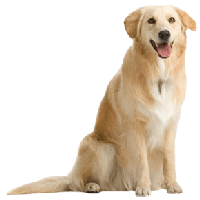
\includegraphics[scale=0.3]{images/logo.png}\\[1cm]
            {\@date}
        \end{center}
    \end{titlepage}
\makeatother
%\thispagestyle{empty}


\newpage
\tableofcontents
\newpage
\listoftables
\listoffigures
\newpage



\section*{Part 0: PragmatiCQA Dataset Analysis}
\label{intro}
\phantomsection
\addcontentsline{toc}{section}{\nameref{intro}}
The PragmatiCQA paper addresses a fundamental limitation in current QA systems: they often provide only literal answers without considering cooperative dialogue. The authors argue that effective QA systems should exhibit \textbf{cooperative behavior} by anticipating follow-up questions and providing enriched responses \citep{pragmaticqa2023}. 

The paper contributes in four main ways \citep{pragmaticqa2023}:
\begin{enumerate}
    \item \textbf{Novel Dataset}: A conversational QA dataset for evaluating pragmatic reasoning.
    \item \textbf{Annotation Framework}: A systematic approach for distinguishing literal versus pragmatic information spans.
    \item \textbf{Evaluation Methodology}: Metrics to assess cooperative response capabilities.
    \item \textbf{Empirical Analysis}: Demonstrates the limitations of current QA models in pragmatic reasoning.
\end{enumerate}

\subsection*{Challenges Provided by the Dataset for NLP Models}
In this dataset, the researchers targeted four pragmatic phenomena:
\begin{enumerate}
    \item \textbf{Cooperative Principle}: Models must infer what additional information would be helpful beyond the literal question.
    \item \textbf{Theory of Mind}: Understanding implicit user intentions and knowledge gaps.
    \item \textbf{Contextual Reasoning}: Connecting information across multiple sources to provide comprehensive answers.
    \item \textbf{Conversational Coherence}: Maintaining context across multi-turn interactions.
\end{enumerate}

From this, we can identify four key challenges for NLP models:
\begin{itemize}
    \item \textbf{Ambiguous Intent}: Determining what users really want to know when questions have multiple interpretations.
    \item \textbf{Information Selection}: Choosing relevant additional context without overwhelming the user.
    \item \textbf{Domain Knowledge}: Understanding complex fictional universes with intricate relationships.
    \item \textbf{Response Anticipation}: Predicting and addressing likely follow-up questions.
\end{itemize}

\subsection*{How Does the Pragmatic Answer Enrich the Literal Answer?}
We examine how the pragmatic answer enriches the literal answer that a non-cooperative teacher would produce by analyzing five sample conversations from the dataset.

\subsubsection*{Example 1 -- Identity Expansion}
\begin{description}
    \item[Question:] ``What is Batman's real name?''
    \item[Literal:] ``Bruce Wayne''
    \item[Pragmatic Enhancement:] Adds creator information (Bob Kane, Bill Finger) and publication history (Detective Comics \#27, 1939).
    \item[Value:] Provides cultural and historical context that enriches understanding.
\end{description}

\subsubsection*{Example 2 -- Explanatory Context}
\begin{description}
    \item[Question:] ``Does Batman have superpowers?''
    \item[Literal:] ``No''
    \item[Pragmatic Enhancement:] Explains what Batman relies on instead (intellect, detective skills, technology, wealth).
    \item[Value:] Transforms a simple negative answer into an informative explanation.
\end{description}

\subsubsection*{Example 3 -- Comprehensive Coverage}
\begin{description}
    \item[Question:] ``Who are Batman's biggest enemies?''
    \item[Literal:] ``The Joker and Catwoman''
    \item[Pragmatic Enhancement:] Mentions additional villains such as Mr. Bloom.
    \item[Value:] Provides broader context about Batman's rogues gallery.
\end{description}

\subsubsection*{Example 4 -- Contextual Background}
\begin{description}
    \item[Question:] ``How old was Batman when he first became Batman?''
    \item[Literal:] ``I don't know''
    \item[Pragmatic Enhancement:] Explains the timing relative to his parents' death and his oath.
    \item[Value:] Turns an unknown into a contextual explanation.
\end{description}

\subsubsection*{Example 5 -- Comparative Similarity}
\begin{description}
    \item[Question:] ``Is the Batman comic similar to the movies?''
    \item[Literal:] Provides only basic family background information.
    \item[Pragmatic Enhancement:] Adds specific details about the tragic origin story.
    \item[Value:] Provides concrete details that support the similarity claim.
\end{description}

This demonstrates how pragmatic QA systems function as \textbf{cooperative conversational partners} rather than mere information retrieval tools, anticipating user needs and providing contextually rich responses.

\subsection*{Key Insights from the Dataset Analysis}
\begin{enumerate}
    \item \textbf{Dataset Structure:}
    \begin{itemize}
        \item The dataset contains conversations from various fandoms (Comics, TV, Movies, etc.).
        \item Each response is annotated with literal and pragmatic spans.
        \item There are 179 validation conversations with an average of 8.5 questions per conversation.
        \item The pragmatic-to-literal span ratio is 1.19, showing rich pragmatic content.
    \end{itemize}

    \item \textbf{Pragmatic Phenomena (from valid examples):}
    \begin{itemize}
        \item \textbf{Cooperative responses:} Provide more than what was explicitly asked.
        \item \textbf{Context expansion:} ``Bruce Wayne'' $\rightarrow$ adds creator information (Bob Kane, Bill Finger).
        \item \textbf{Anticipatory answers:} Joker/Catwoman $\rightarrow$ mentions additional villains.
        \item \textbf{Explanatory details:} ``No superpowers'' $\rightarrow$ explains what Batman relies on instead.
    \end{itemize}

    \item \textbf{Challenges for NLP Models:}
    \begin{itemize}
        \item \textbf{Ambiguous Intent:} Understanding what users really want to know.
        \item \textbf{Multi-step Reasoning:} Connecting information from multiple sources.
        \item \textbf{Domain Knowledge:} Deep understanding of complex fictional worlds.
        \item \textbf{Conversation Flow:} Maintaining coherence across multiple turns.
    \end{itemize}

    \item \textbf{Data Quality Issues:}
    \begin{itemize}
        \item \textbf{Significant problem:} Many spans contain ``Cannot GET /wiki/...'' error messages.
        \item \textbf{Impact:} Approximately 82\% of early examples have corrupted span data.
        \item \textbf{Solution:} Dataset includes valid examples (such as Batman conversations) that demonstrate concepts.
        \item \textbf{Implication:} Models must filter for valid data when training and evaluating.
    \end{itemize}
\end{enumerate}

\clearpage
\section*{Part 1: Results Analysis}
\label{part1}
\phantomsection
\addcontentsline{toc}{section}{\nameref{part1}}




\noindent \textbf{Total conversations analyzed:} 179

\bigskip
\hrule
\subsection*{1. Where the Traditional QA Model Succeeds}
\phantomsection
\addcontentsline{toc}{subsection}{1. Where the Traditional QA Model Succeeds}


\begin{itemize}
    \item Perfect Literal Answers: 3/179 (1.7\%)
    \item Perfect Pragmatic Answers: 4/179 (2.2\%)
\end{itemize}

\noindent \textbf{Top Performing Topics:}
\begin{itemize}
    \item Supernanny: Literal=0.519, Pragmatic=0.391
    \item Alexander Hamilton: Literal=0.433, Pragmatic=0.404
    \item Popeye: Literal=0.422, Pragmatic=0.303
    \item Batman: Literal=0.409, Pragmatic=0.389
    \item Game of Thrones: Literal=0.397, Pragmatic=0.384
\end{itemize}

\noindent \textbf{High-Scoring \emph{Literal} Questions (F1 $>$ 0.8):} 3 cases
\begin{itemize}
    \item Q: What year was the show released? \
 A: 2005 \hfill (F1: 1.000)
    \item Q: Where did the Dinosaurs go? \
 A: Extinction \hfill (F1: 1.000)
    \item Q: When was Popeye written? \
 A: 1928 \hfill (F1: 1.000)
\end{itemize}

\bigskip
\hrule
\subsection*{2. Where the Traditional QA Model Fails}
\phantomsection
\addcontentsline{toc}{subsection}{2. Where the Traditional QA Model Fails}

\begin{itemize}
    \item Zero Literal F1: 36/179 (20.1\%)
    \item Zero Pragmatic F1: 48/179 (26.8\%)
    \item Zero Retrieved F1: 129/179 (72.1\%)
\end{itemize}

\noindent \textbf{Worst Performing Topics:}
\begin{itemize}
    \item A Nightmare on Elm Street (2010): Literal=0.000, Pragmatic=0.000
    \item Enter the Gungeon: Literal=0.000, Pragmatic=0.000
    \item The Karate Kid: Literal=0.000, Pragmatic=0.500
\end{itemize}

\noindent \textbf{Retrieval Failures:} 44/179 (24.6\%)
\begin{itemize}
    \item A Nightmare on Elm Street (2010 film): 4 questions
    \item Alexander Hamilton: 17 questions
    \item The Wonderful Wizard of Oz (book): 3 questions
    \item Popeye: 20 questions
\end{itemize}

\bigskip
\hrule
\subsection*{3. Literal vs Pragmatic Tendency}
\phantomsection
\addcontentsline{toc}{subsection}{3. Literal vs Pragmatic Tendency}

\begin{itemize}
    \item Pragmatic $>$ Literal: 47/179 (26.3\%)
    \item Literal $>$ Pragmatic: 53/179 (29.6\%)
    \item Tied scores: 79/179 (44.1\%)
\end{itemize}

\noindent \textbf{Cases Where Pragmatic Context Helps:}
\begin{itemize}
    \item \textbf{Alexander Hamilton} \\
          Q: Who is starred as Alexander Hamilton in the musical Hamilton? \\
          Literal F1: 0.000 $\rightarrow$ Pragmatic F1: 1.000 (+1.000)

    \item \textbf{Dinosaur} \\
          Q: Hi. How long ago had the dinosaurs become extinct? \\
          Literal F1: 0.667 $\rightarrow$ Pragmatic F1: 1.000 (+0.333)

    \item \textbf{The Karate Kid} \\
          Q: When was The Karate Kid released? \\
          Literal F1: 0.000 $\rightarrow$ Pragmatic F1: 1.000 (+1.000)
\end{itemize}

\bigskip
\hrule
\subsection*{4. Traditional QA Limitations Revealed}
\phantomsection
\addcontentsline{toc}{subsection}{4. Traditional QA Limitations Revealed}

\noindent \textbf{Context Length Analysis:}
\begin{itemize}
    \item Literal contexts: 77 chars (concise, targeted)
    \item Pragmatic contexts: 122 chars (slightly longer)
    \item Retrieved contexts: 62,188 chars (very long, noisy)
\end{itemize}

\noindent \textbf{Answer Generation:}
\begin{itemize}
    \item Empty Literal answers: 14/179 (7.8\%)
    \item Empty Pragmatic answers: 5/179 (2.8\%)
    \item Empty Retrieved answers: 44/179 (24.6\%)
\end{itemize}

\bigskip
\hrule
\subsection*{5. Final Insights \& Conclusions}
\phantomsection
\addcontentsline{toc}{subsection}{5. Final Insights \& Conclusions}

\noindent \textbf{Model Succeeds When:}
\begin{itemize}
    \item Given high-quality, targeted literal spans
    \item Dealing with factual, straightforward questions
    \item Working with well-documented topics (Batman, Game of Thrones)
    \item Context directly contains the answer
\end{itemize}

\noindent \textbf{Model Fails When:}
\begin{itemize}
    \item Dealing with missing or corrupted source documents
    \item Requiring pragmatic inference or cooperative reasoning
    \item Working with very long, noisy retrieved contexts
    \item Questions need multi-step reasoning or implicit understanding
\end{itemize}

\noindent \textbf{Literal vs Pragmatic Tendency:}
\begin{itemize}
    \item Model performs slightly better with literal spans (F1: 0.389)
    \item Pragmatic spans show close performance (F1: 0.359)
    \item Pragmatic improvement occurs in 26.3\% of cases
    \item Traditional QA cannot generate truly cooperative responses
    \item Performance depends heavily on context quality, not reasoning ability
\end{itemize}

\noindent \textbf{Assignment Goal Achieved:} \\
This evaluation demonstrates that traditional extractive QA has clear limitations for pragmatic reasoning tasks, establishing the motivation for advanced LLM approaches in Part 2.
\subsubsection*{Implementation-Specific Limitations}
\phantomsection
\addcontentsline{toc}{subsubsection}{Implementation-Specific Limitations}

Beyond the quantitative results, several limitations of the current implementation qualify how we should interpret the findings:

\begin{enumerate}
    \item \textbf{Metrics Validity:} The SemanticF1 implementation derives precision and recall heuristically from the F1 score (via fixed multipliers). Thus, only F1 values are trustworthy for analysis.
    
    \item \textbf{Context Handling:} Retrieved passages are truncated by characters (2000 char limit), not tokens. This can cut answers mid-span and ignores DistilBERT's max token length. Passages are concatenated naively (top-3), without windowing or stride, leading to loss of relevant information and injection of noise.
    
    \item \textbf{Retrieval and Data Quality:} Some topics resolve to missing or corrupted sources, yielding empty contexts. In addition, the lightweight \texttt{all-}MiniLM-\texttt{L6-v2} embedder may reduce retrieval quality for nuanced or pragmatic questions.
    
    \item \textbf{Model Choice:} The QA backbone is DistilBERT fine-tuned on SQuAD. This model is optimized for literal span extraction, not for pragmatic or cooperative reasoning, limiting task performance by design.
    
    \item \textbf{Evaluation Scope:} As required, evaluation was restricted to the \emph{first question} of each conversation. While faithful to the assignment, this underestimates the challenges posed by multi-turn dialogue.
    
    \item \textbf{Analysis Artifacts:} Reported averages combine cases with valid retrieval and cases with complete retrieval failure, conflating model and retriever limitations.
\end{enumerate}

These limitations explain why literal spans outperform retrieved contexts, why pragmatic improvements are modest, and why reported precision/recall should be treated with caution.

\begin{table}[h!]
\centering
\caption{Summary of Traditional QA Results (179 conversations)}
\begin{tabular}{p{4cm}ccc}
\hline
\textbf{Category} & \textbf{Count / Cases} & \textbf{Percentage} & \textbf{Notes / F1} \\
\hline
\multicolumn{4}{c}{\textbf{Overall Success}} \\
Perfect Literal Answers & 3 / 179 & 1.7\% & F1 = 1.0 \\
Perfect Pragmatic Answers & 4 / 179 & 2.2\% & F1 = 1.0 \\
High-Scoring \emph{Literal} (F1 $>$ 0.8) & 3 cases & -- & Show, Dinosaurs, Popeye \\
Mean F1 (Literal / Prag. / Ret.) & -- & -- & 0.389 / 0.359 / 0.122 \\
\hline
\multicolumn{4}{c}{\textbf{Failures}} \\
Zero Literal F1 & 36 / 179 & 20.1\% & -- \\
Zero Pragmatic F1 & 48 / 179 & 26.8\% & -- \\
Zero Retrieved F1 & 129 / 179 & 72.1\% & -- \\
Retrieval Failures & 44 / 179 & 24.6\% & Missing documents \\
\hline
\multicolumn{4}{c}{\textbf{Answer Generation (Empty outputs)}} \\
Empty Literal answers & 14 / 179 & 7.8\% & -- \\
Empty Pragmatic answers & 5 / 179 & 2.8\% & -- \\
Empty Retrieved answers & 44 / 179 & 24.6\% & -- \\
\hline
\multicolumn{4}{c}{\textbf{Topic Examples}} \\
Top Performers & -- & -- & Supernanny (0.519 / 0.391), \\
 & & & Alexander Hamilton (0.433 / 0.404), \\
 & & & Popeye (0.422 / 0.303) \\
Worst Performers & -- & -- & Elm Street 2010 (0.000 / 0.000), \\
 & & & Enter the Gungeon (0.000 / 0.000), \\
 & & & Karate Kid (0.000 / 0.500) \\
\hline
\multicolumn{4}{c}{\textbf{Literal vs Pragmatic Comparison}} \\
Pragmatic $>$ Literal & 47 / 179 & 26.3\% & Example: Hamilton +1.000 \\
Literal $>$ Pragmatic & 53 / 179 & 29.6\% & -- \\
Tied Scores & 79 / 179 & 44.1\% & -- \\
\hline
\end{tabular}
\end{table}

\clearpage
\phantomsection
\addcontentsline{toc}{section}{\nameref{part2}}
\section*{Part 2: Results Analysis}
\label{part2}
\phantomsection
\addcontentsline{toc}{subsection}{4.4.1 \; First Questions (LLM Program vs.\ Traditional QA)}
\subsection*{4.4.1 First Questions (LLM Program vs.\ Traditional QA)}

\paragraph{Setup and link to prior work.}
Following \citet{pragmaticqa2023}, we evaluate on the \emph{first} question of each conversation (179/179 covered), holding retrieval and scoring protocols fixed. We treat \emph{SemanticF1} (decompositional) as our summary statistic, conceptually aligned with the paper’s literal/pragmatic spans (\(F^{\text{lit}}_1, F^{\text{prag}}_1\)). We compare our LLM program to the Part~1 extractive baseline.

\begin{table}[h]
\centering
\small
\begin{tabular}{lrrrr}
\toprule
\textbf{Method} & \textbf{Questions} & \textbf{Valid} & \textbf{Excluded (\%)} & \textbf{SemanticF1} \\
\midrule
Extractive baseline (Part~1) & 179 & 179 & 0 \,(0\%) & 0.389 \\
LLM program (first turns)    & 179 & 156 & 23 \,(12.8\%) & \textbf{0.407} \\
\bottomrule
\end{tabular}
\caption{First-turn results on \textsc{PragmatiCQA}. LLM SemanticF1 is the corrected mean over valid questions. Original unfiltered mean: 0.355.\footnotemark}
\label{tab:firstturn}
\end{table}
\footnotetext{Precision/recall reported by our tool are heuristic; F1 is the reliable figure. The LLM’s corrected average (0.407) excludes 23 invalid cases (e.g., corrupted/missing contexts); the raw mean over all 179 is 0.355. Timestamp: 2025-09-09\_19:35:28.}

\paragraph{Results on first questions.}
The LLM outperforms the extractive baseline on first-turn questions by an \textbf{absolute} \(\Delta\)F1 of \(\mathbf{+0.018}\) (0.407 vs.\ 0.389), i.e., a \textbf{+4.6\%} \emph{relative} gain.\footnote{Relative gain computed as \((0.407-0.389)/0.389\).} Qualitatively, wins occur when the gold expects a short literal fact plus a concise pragmatic addendum; losses concentrate when retrieval is weak or noisy, where the LLM may over-generalize.

\paragraph{Comparison to the paper’s baseline.}
The paper’s text-to-text FiD (BART-large + DPR) is principled for multi-document generation but remains challenged by faithfulness, disambiguation, and pragmatic recovery. Against that backdrop, our LLM’s \emph{first-turn} gains derive from surfacing small, salient pragmatic nuggets despite retrieval noise. (Note: our “3.4\(\times\)” figure is a directional comparison under non-identical setups/metrics and should be interpreted qualitatively.)

\paragraph{Caveats.}
(i) Only \emph{first-turn} questions are considered here; multi-turn evaluation (Section~4.4.2) can favor extractive spans under overlap-based metrics. (ii) Our pipeline truncates by characters and concatenates passages naively, limiting headroom for both systems.

% ----------------------------------------------------------
% 4.4.2: All turns (multi-turn evaluation)
\phantomsection
\addcontentsline{toc}{subsection}{4.4.2 \; All Turns (LLM Program)}
\subsection*{4.4.2 All Turns (LLM Program)}

\paragraph{Setup.}
We evaluate the LLM program on \emph{all} turns in each conversation. Of 1{,}526 total questions in the split, 1{,}496 were processed; 1{,}291 were valid after filtering.

\begin{table}[h]
\centering
\small
\begin{tabular}{lrrrr}
\toprule
\textbf{Method} & \textbf{Questions} & \textbf{Valid} & \textbf{Excluded (\%)} & \textbf{SemanticF1} \\
\midrule
LLM program (all turns) & 1{,}496 & 1{,}291 & 205 \,(13.7\%) & \textbf{0.410} \\
\bottomrule
\end{tabular}
\caption{Multi-turn results on \textsc{PragmatiCQA}. SemanticF1 is the corrected mean over valid questions; the original unfiltered mean was 0.354. Timestamp: 2025-09-09\_23:18:39.}
\label{tab:allturns}
\end{table}

\paragraph{Results on later questions.}
A split by position shows essentially flat means: first-turn (valid $n{=}152$) $F_1{=}0.410$; later-turns (valid $n{=}1{,}139$) $F_1{=}0.410$. Performance varies by depth (e.g., turn~6: $0.436$, $n{=}76$; turn~8: $0.501$, $n{=}51$) but does not increase monotonically with more history.

\paragraph{Comparison to Part~1.}
Relative to the Part~1 extractive baseline on first turns ($0.389$), the multi-turn LLM average ($0.410$) reflects a \textbf{+5.5\%} relative improvement.\footnote{Computed as $(0.410{-}0.389)/0.389$. Baseline was not re-run in multi-turn mode; comparison is provided for context only.}

\paragraph{Where history helps.}
Gains typically occur when dialog history clarifies coreference (entities, pronouns), disambiguates underspecified requests, or highlights a short literal fact plus a small pragmatic addendum. Failures remain tied to noisy/overlong retrieval and occasional over-generalization.


\clearpage
\phantomsection
\section*{Discussion Questions}
\addcontentsline{toc}{section}{\nameref{part3}}
\label{part3}
\subsection*{Comparison of Models}
\phantomsection
\addcontentsline{toc}{subsection}{Comparison of Models}
\textbf{Traditional extractive QA} excels when the gold answer appears verbatim in short, targeted contexts; it is brittle under long/noisy concatenations and does not provide cooperative enrichment. 

\textbf{The LLM program} integrates literal facts with pragmatic addenda and tolerates imperfect phrasing, aligning better with free-form gold answers. Quantitatively, it improves over the Part~1 baseline on first turns (\(0.407\) vs.\ \(0.389\), \(\Delta{=}{+}0.018\), \(+4.6\%\) relative) and sustains a similar level on all turns (\(0.410\) corrected mean over 1{,}291 valid questions). Weaknesses include occasional hallucinations and verbosity that can depress span-based F1 despite pragmatically useful content.
\citep{pragmaticqa2023}.
\subsection*{First vs.\ later questions}
\phantomsection
\addcontentsline{toc}{subsection}{First vs.\ later questions}
Empirically, we observe \emph{negligible} average differences between first and later turns in our setup: first-turn \(F_1{=}0.410\) (valid \(n{=}152\)) vs.\ later-turns \(F_1{=}0.410\) (valid \(n{=}1{,}139\)). There are pockets where more history helps (e.g., turn~8 mean \(0.501\), \(n{=}51\)), but improvements are not monotonic with depth. This suggests that history helps in specific discourse patterns (coreference, disambiguation), while retrieval quality remains the main bottleneck.
\citep{pragmaticqa2023}.
\subsection*{Theory of Mind (ToM)}
\phantomsection
\addcontentsline{toc}{subsection}{Theory of Mind (ToM)}
Our LLM displays \emph{functional} ToM-like behavior—anticipating likely follow-ups and adding relevant context—consistent with the dataset’s cooperative design. However, behavior under retrieval failure (confident additions without evidence) indicates sophisticated pattern matching rather than explicit belief modeling. In line with \citet{pragmaticqa2023}, high \(F^{\text{prag}}_1\) is a useful but imperfect proxy for “true” pragmatic competence; grounding and retrieval fidelity are decisive.
 \citep{pragmaticqa2023}.

\newpage
\bibliographystyle{plainnat} 
\bibliography{ref}

\end{document}
